%%%%%%%%%%%%%%%%%%%%%%%%%%%%%%%%%%%%%%%%%%%%%%%%%%%%%%%%%%%%%%%%%%%%%%
% Overleaf (WriteLaTeX) Example: Molecular Chemistry Presentation
%
% Source: http://www.overleaf.com
%
% In these slides we show how Overleaf can be used with standard
% chemistry packages to easily create professional presentations.
%
% Feel free to distribute this example, but please keep the referral
% to overleaf.com
%
%%%%%%%%%%%%%%%%%%%%%%%%%%%%%%%%%%%%%%%%%%%%%%%%%%%%%%%%%%%%%%%%%%%%%%

\documentclass[xcolor={dvipsnames}]{beamer}

\mode<presentation>
{
  \usetheme{Madrid}       % or try default, Darmstadt, Warsaw, ...
  \usecolortheme{default} % or try albatross, beaver, crane, ...
  \usefonttheme{default}    % or try default, structurebold, ...
  \setbeamertemplate{navigation symbols}{}
  \setbeamertemplate{caption}[numbered]
}

\usepackage[english]{babel}
\usepackage[utf8x]{inputenc}
\usepackage{graphicx}
\usepackage{hyperref}
  \hypersetup{colorlinks=true}
  \hypersetup{urlcolor=blue}
  \hypersetup{linkcolor = .}
\usepackage{xcolor}
\usepackage{siunitx}
  \sisetup{separate-uncertainty = true}
\DeclareSIUnit\barn{b}
\usepackage{physics}
\usepackage[font=small,labelfont=bf]{caption}
\usepackage{subcaption}
\usepackage[en-GB]{datetime2}
\usepackage{overpic}
\usepackage{feynmp}
\DeclareGraphicsRule{*}{mps}{*}{}
\usepackage{scalerel}
\newcommand{\mylbrace}[2]{\vspace{#2pt}\hspace{6pt}\scaleleftright[\dimexpr5pt+#1\dimexpr0.06pt]{\lbrace}{\rule[\dimexpr2pt-#1\dimexpr0.5pt]{-4pt}{#1pt}}{.}}
\newcommand{\myrbrace}[2]{\vspace{#2pt}\scaleleftright[\dimexpr5pt+#1\dimexpr0.06pt]{.}{\rule[\dimexpr2pt-#1\dimexpr0.5pt]{-4pt}{#1pt}}{\rbrace}\hspace{6pt}}

% Trim in percent
\usepackage{adjustbox}

% No "Figure" prefix
\setbeamertemplate{caption}{\raggedright\insertcaption\par}

% Nice decay amplitude diagrams
\usepackage{amsmath,amssymb,tikz-cd}

% Strike out text
\usepackage[normalem]{ulem}

% For figures with text overlay
\usepackage{overpic}

% Arrows
\usepackage{tikz}
\newcommand{\tikzmark}[1]{\tikz[remember picture] \node[coordinate] (#1) {#1};}

% Colourbox with line breaks
\newcommand{\cbox}[2][lime!20]{%
  \colorbox{#1}{\parbox{\dimexpr\linewidth-2\fboxsep}{\strut #2\strut}}%
}

% Vector arrows
\usepackage[pdftex]{pict2e}

% Checkmark symbol
\def\checkmark{\tikz\fill[scale=0.4](0,.35) -- (.25,0) -- (1,.7) -- (.25,.15) -- cycle;}

% Here's where the presentation starts, with the info for the title slide
\title[Heidelberg tracking meeting]{Understanding discrepancies in tracking efficiencies}

\author[Martin Tat]{Martin Tat}
\institute[Heidelberg]{Heidelberg University}
\date{13th August 2025}

\titlegraphic{
\includegraphics[height = 2.3cm]{lhcb.jpg}\hspace{1.0cm}~%
              
\includegraphics[height = 2.3cm]{HeidelbergLogo.pdf}}

\begin{document}

\begin{frame}
  \titlepage
\end{frame}

% These three lines create an automatically generated table of contents.
%\begin{frame}{Outline}
%  \tableofcontents
%\end{frame}

\begin{frame}{Introduction}
  \vspace{0.0cm}
  {\Large Recap from last time:}
  \vspace{0.2cm}
  \begin{itemize}
    \setlength\itemsep{0.8em}
    \item{Had a look at tracking efficiencies using TrackCalib2}
    \item{Fits to MC}
    \item{Studied fit biases}
    \begin{enumerate}
      \item{In some bins the uncertainties were underestimated}
      \item{Improve by changing background parameterisation}
      \item{$(N_{\rm tot}, \epsilon_{\rm track})\to(N_{\rm matched}, N_{\rm failed})$ for background yields}
    \end{enumerate}
    \item{Today:}
    \begin{enumerate}
      \item{Some developments to TrackCalib2}
      \item{Further tweaks to stabilise fits and reduce fit biases}
      \item{Fits to data}
    \end{enumerate}
  \end{itemize}
\end{frame}

\begin{frame}{Tag-and-probe method}
  \vspace{0.0cm}
  \begin{figure}[htb]
    \centering
    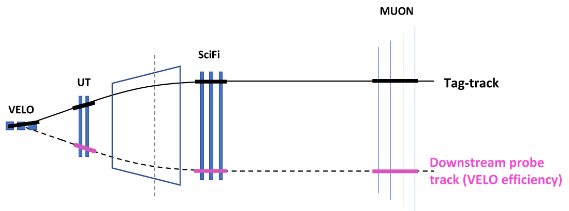
\includegraphics[width=0.75\textwidth]{Plots/Tag_and_probe_method.png}
    \caption*{\small Figure from \href{https://www.physi.uni-heidelberg.de/Publications/PhD_thesis.pdf}{Rowina's thesis}}
  \end{figure}
  \begin{itemize}
    \item{Fully reconstruct one muon from $J/\psi\to\mu^+\mu^-$}
    \item{Partially reconstruct the other muon}
    \item{Match hits in specific sub-detector with partially reconstructed track}
  \end{itemize}
  \begin{equation*}
    \epsilon_{\rm track} = \frac{N_{\rm matched}}{N_{\rm matched} + N_{\rm failed}}
  \end{equation*}
\end{frame}

\begin{frame}{Tweaks to TrackCalib2}
  \vspace{0.0cm}
  \begin{itemize}
    \setlength\itemsep{1.0em}
    \item{TrackCalib2 works well out-of-the-box}
    \item{But I wanted to make a few changes, after my studies on fit biases}
    \begin{itemize}
      \item{TrackCalib2 developments in the \texttt{mtat/dev/2024} branch}
      \item{TCFit developments still local, no push access yet}
    \end{itemize}
    \item{Improvements are mainly to stabilise the fit and ensure good convergence}
  \end{itemize}
\end{frame}

\begin{frame}{TrackCalib2 tweak 1}
  \vspace{0.0cm}
  \begin{center}
    {\large Changed background yield parameterisation}
  \end{center}
  \vspace{0.5cm}
  \begin{itemize}
    \setlength\itemsep{1.0em}
    \item{$(N_{\rm tot}, \epsilon_{\rm track})\to(N_{\rm matched}, N_{\rm failed})$}
    \item{Some efficiencies and uncertainties have moved slightly}
    \begin{itemize}
      \item{Particularly important in bins where the signal yield in the failed sample is very small}
    \end{itemize}
  \end{itemize}
\end{frame}

\begin{frame}{TrackCalib2 tweak 2}
  \vspace{0.0cm}
  \begin{center}
    {\large Change from exponential to Chebyshev polynomial for background shape}
  \end{center}
  \vspace{0.5cm}
  \begin{itemize}
    \setlength\itemsep{1.0em}
    \item{Exponential shape doesn't describe background well, especially in data}
    \item{TrackCalib2 by default uses Chebyshev polynomials of order $3$, with separate shapes for matched and failed samples}
    \begin{itemize}
      \item{$\to$ Change to second order for failed sample}
    \end{itemize}
    \item{Improves fit quality, but also makes it slower and perhaps more unstable because it adds $4$ additional parameters}
  \end{itemize}
\end{frame}

\begin{frame}{TrackCalib2 tweak 3}
  \vspace{0.0cm}
  \begin{center}
    {\large Change parameterisation of the widths $\sigma$}
  \end{center}
  \vspace{0.5cm}
  \begin{itemize}
    \setlength\itemsep{1.0em}
    \item{Matched signal shape is two Crystal Ball functions with different $\sigma$}
    \item{Failed signal shape also has two Crystal Ball functions, where one of the $\sigma$ are shared with the matched shape}
    \item{In total $3$ different $\sigma$ parameters $\to$ Can lead to degeneracies and unstable fits, especially in data}
    \item{Instead I changed it to $\sigma^\prime = R\sigma$ where the ratio $R$ is floating}
    \begin{itemize}
      \item{Can also fix $R$ in the fit to data, so that only a single $\sigma$ parameter is floated in the fit to data}
    \end{itemize}
  \end{itemize}
\end{frame}

\begin{frame}{TrackCalib2 tweak 4}
  \vspace{0.0cm}
  \begin{center}
    {\large Bug fix in Crystal Ball shape}
  \end{center}
  \vspace{0.5cm}
  \begin{itemize}
    \setlength\itemsep{1.0em}
    \item{Two independent bugs in TCFit and RooFit}
    \begin{itemize}
      \item{RooFit bug was only revealed because of TCFit bug!}
    \end{itemize}
    \item{TCFit bug: Exponent $n$ in the power-law tail was forced to be $n > 1$}
    \begin{itemize}
      \item{This restricts the shape to have very small tails, but tails can be large}
      \item{Wikipedia wrongly states that $n > 1$, but this is only true if the range is infinite, for finite ranges we are only restricted by $n > 0$!}
    \end{itemize}
  \end{itemize}
\end{frame}

\begin{frame}{TrackCalib2 tweak 4}
  \vspace{0.0cm}
  \begin{center}
    {\large Bug fix in Crystal Ball shape}
  \end{center}
  \vspace{0.5cm}
  \begin{itemize}
    \setlength\itemsep{1.0em}
    \item{RooFit bug: In a range $n - 1 \in [-10^{-5}, 10^{-5}]$, an approximation must be used in the normalisation integral (with $b = (n/\alpha)^n - \alpha$):}
  \end{itemize}
  \begin{align*}
    &\big(\frac{n}{\alpha}\big)^n\times\frac{(b - z_{\rm min})^{1 - n} - (b + z_{\rm max})^{1 - n}}{1 - n} \\
    \approx &\big(\frac{n}{\alpha}\big)^n\times\big(\ln(b - z_{\rm min}) - \ln(b + z_{\rm max})\big)
  \end{align*}
  \begin{itemize}
    \setlength\itemsep{1.0em}
    \item{This is wrong!}
  \end{itemize}
\end{frame}

\begin{frame}{TrackCalib2 tweak 4}
  \vspace{0.0cm}
  \begin{center}
    {\large Bug fix in Crystal Ball shape}
  \end{center}
  \vspace{0.5cm}
  \begin{align*}
    &\big(\frac{n}{\alpha}\big)^n\times\frac{(b - z_{\rm min})^{1 - n} - (b + z_{\rm max})^{1 - n}}{1 - n} \\
    \approx &\big(\frac{n}{\alpha}\big)^n\times\big(\ln(b - z_{\rm min}) - \ln(b + z_{\rm max})\big)
  \end{align*}
  \begin{itemize}
    \setlength\itemsep{1.0em}
    \item{Prefactor $(n/\alpha)^n$ can be expanded to first order in $n - 1$}
    \item{So numerator must be expanded to \underline{second} order}
  \end{itemize}
  \begin{align*}
    \big(\frac{n}{\alpha}\big)^n\times\big(&\ln(b - z_{\rm min}) - \ln(b + z_{\rm max}) \\
    + &\frac{1}{2}(1 - n)(\ln(b - z_{\rm min})^2 - \ln(b - z_{\rm max})^2)\big)
  \end{align*}
\end{frame}

\begin{frame}{TrackCalib2 tweak 4}
  \vspace{0.0cm}
  \begin{center}
    {\large Bug fix in Crystal Ball shape}
  \end{center}
  \vspace{0.0cm}
  \begin{figure}[htb]
    \centering
    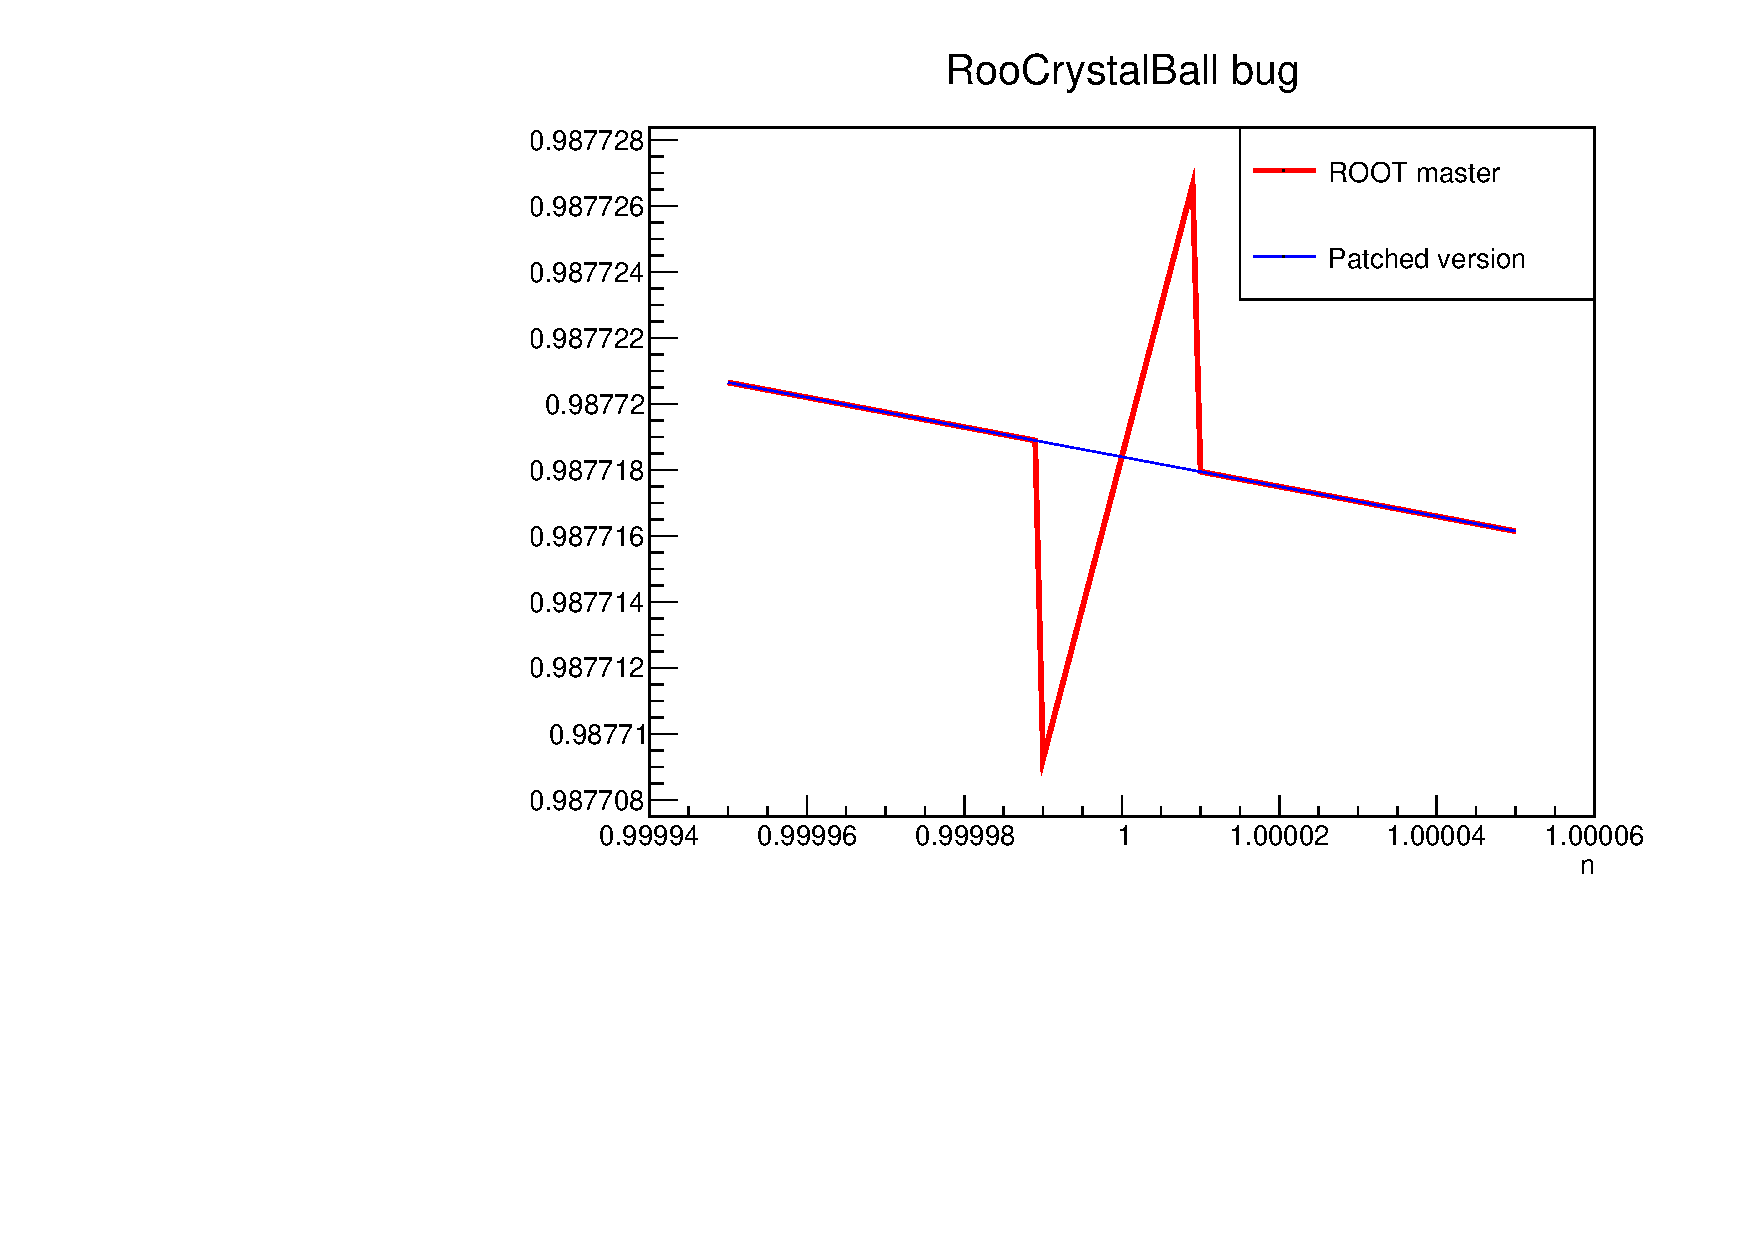
\includegraphics[width=0.4\textwidth]{Plots/RooCrystalBall_fix.pdf}
  \end{figure}
  \vspace{-0.5cm}
  \begin{itemize}
    \setlength\itemsep{0.0em}
    \item{This bug can trick the fit into converging near $n = 1$ with a very small uncertainty}
    \item{I assume it's highly unlikely, and people probably just changed the starting parameters when that happened in the past...}
    \item{... but with the TCFit, it resulted in weird behaviour near $n = 1$}
    \item{Opened a pull request to the ROOT project here: \href{https://github.com/root-project/root/pull/19602}{!19602}}
  \end{itemize}
\end{frame}

\begin{frame}{Tracking efficiencies}
  \vspace{0.0cm}
  \begin{figure}[htb]
    \centering
    \begin{subfigure}{0.5\textwidth}
      \centering
      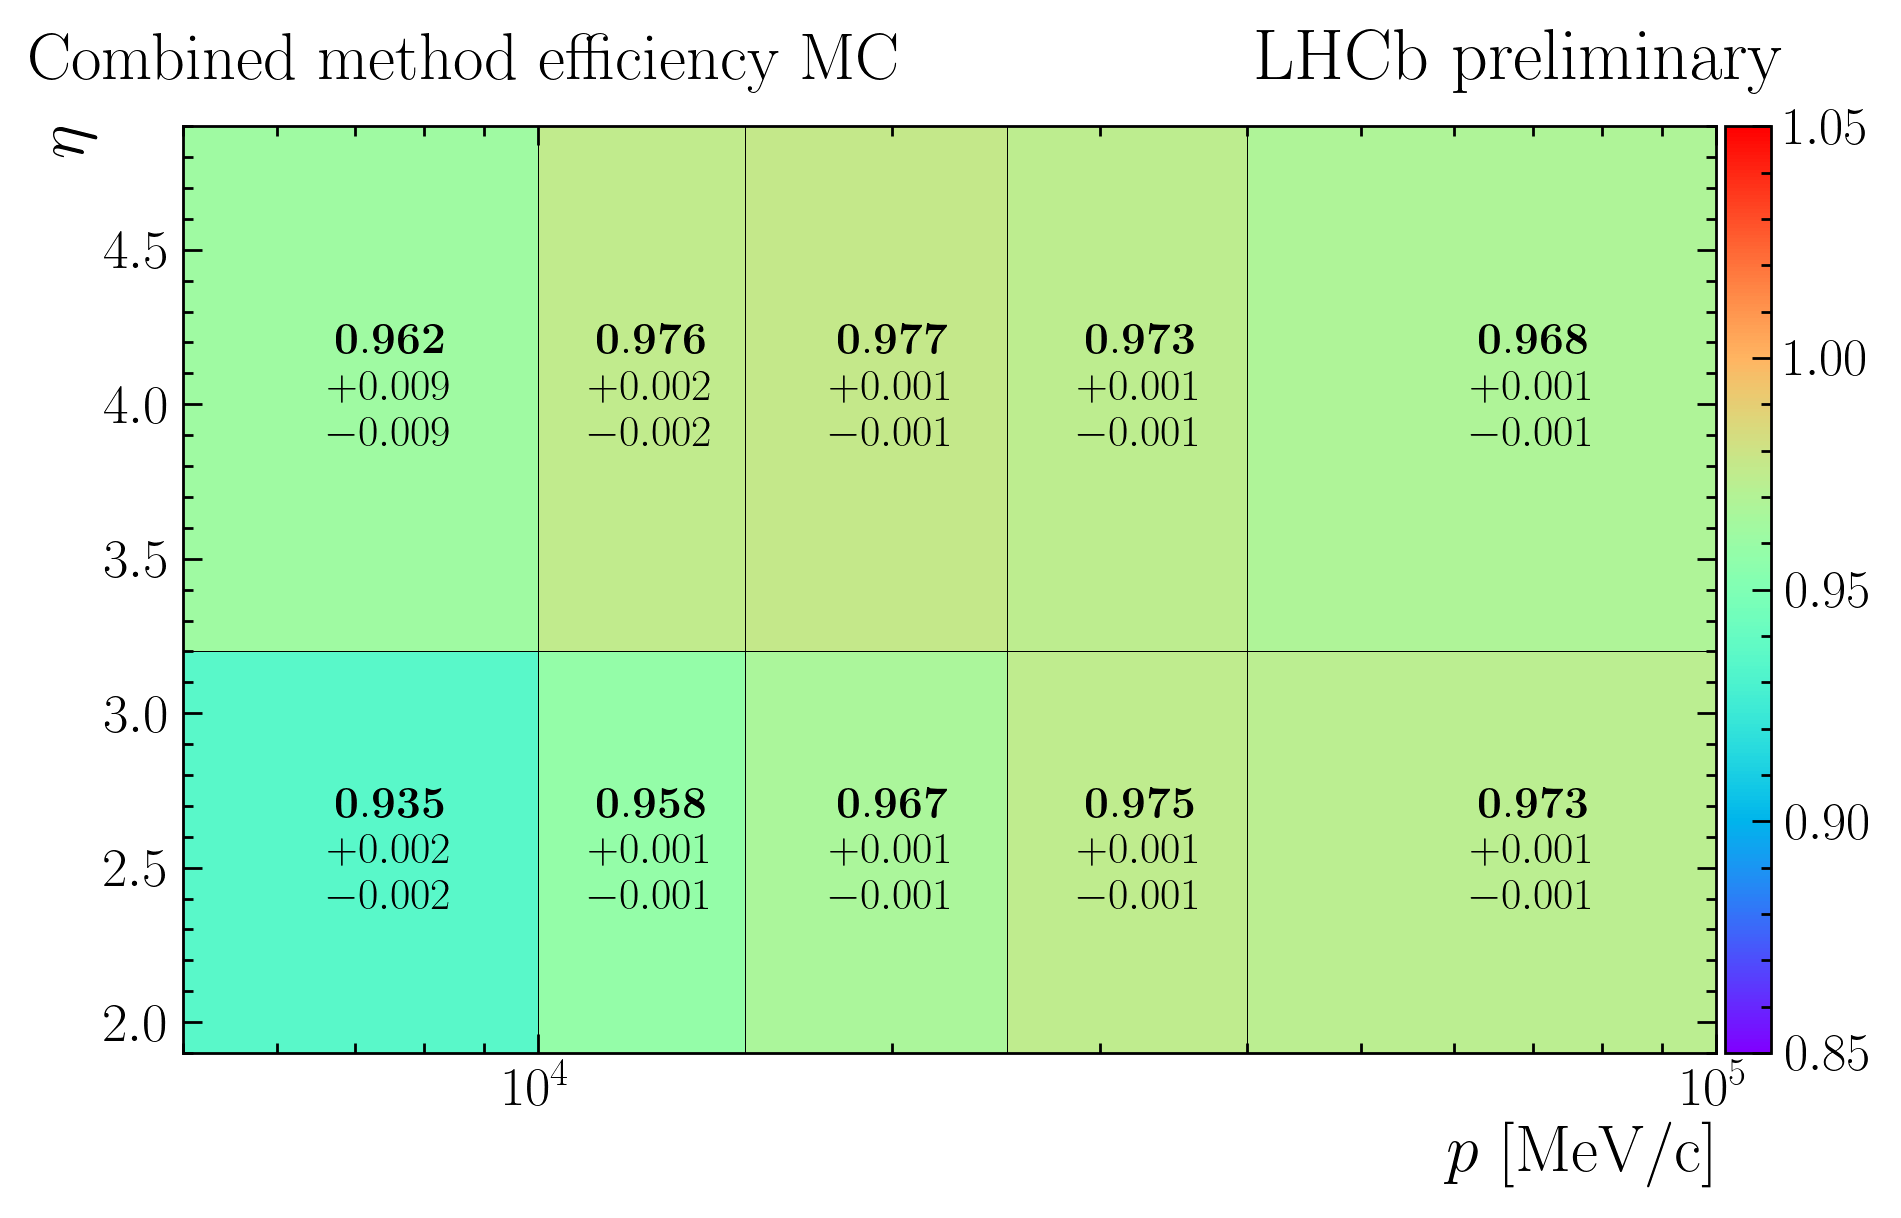
\includegraphics[width=1.0\textwidth]{Plots/trackEff_MC_Sim10d_2024_Block1_Combined_P-ETA.png}
    \end{subfigure}%
    \begin{subfigure}{0.5\textwidth}
      \centering
      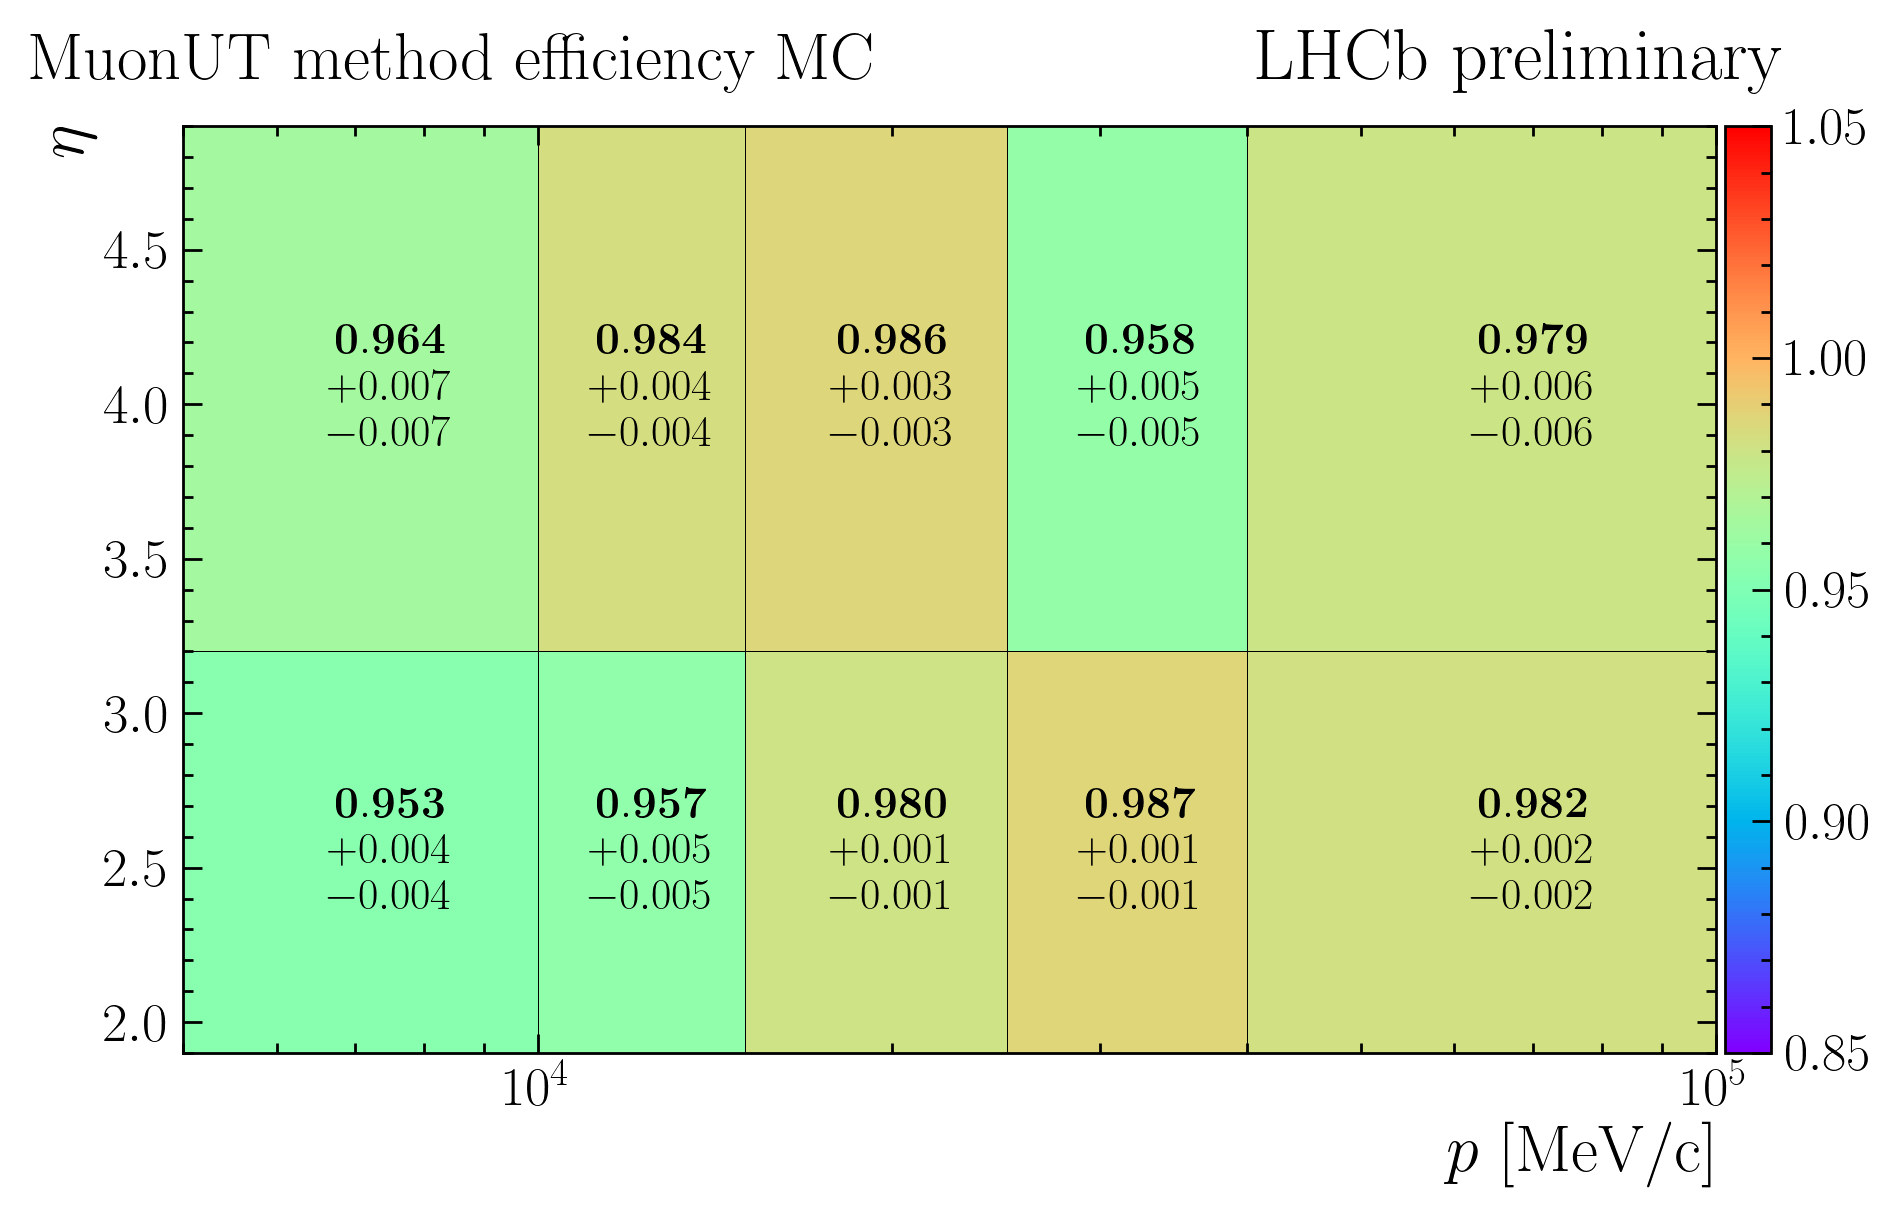
\includegraphics[width=1.0\textwidth]{Plots/trackEff_MC_Sim10d_2024_Block1_MuonUT_P-ETA.png}
    \end{subfigure}
  \end{figure}
  \begin{itemize}
    \item{Discrepancies are roughly $1\%$ between Combined and MuonUT methods}
    \item{Bin $(0, 0)$ has a $(2.2 \pm 0.4)\%$ discrepancy}
  \end{itemize}
\end{frame}

\begin{frame}{Tracking efficiencies}
  \vspace{0.0cm}
  \begin{figure}[htb]
    \centering
    \begin{subfigure}{0.5\textwidth}
      \centering
      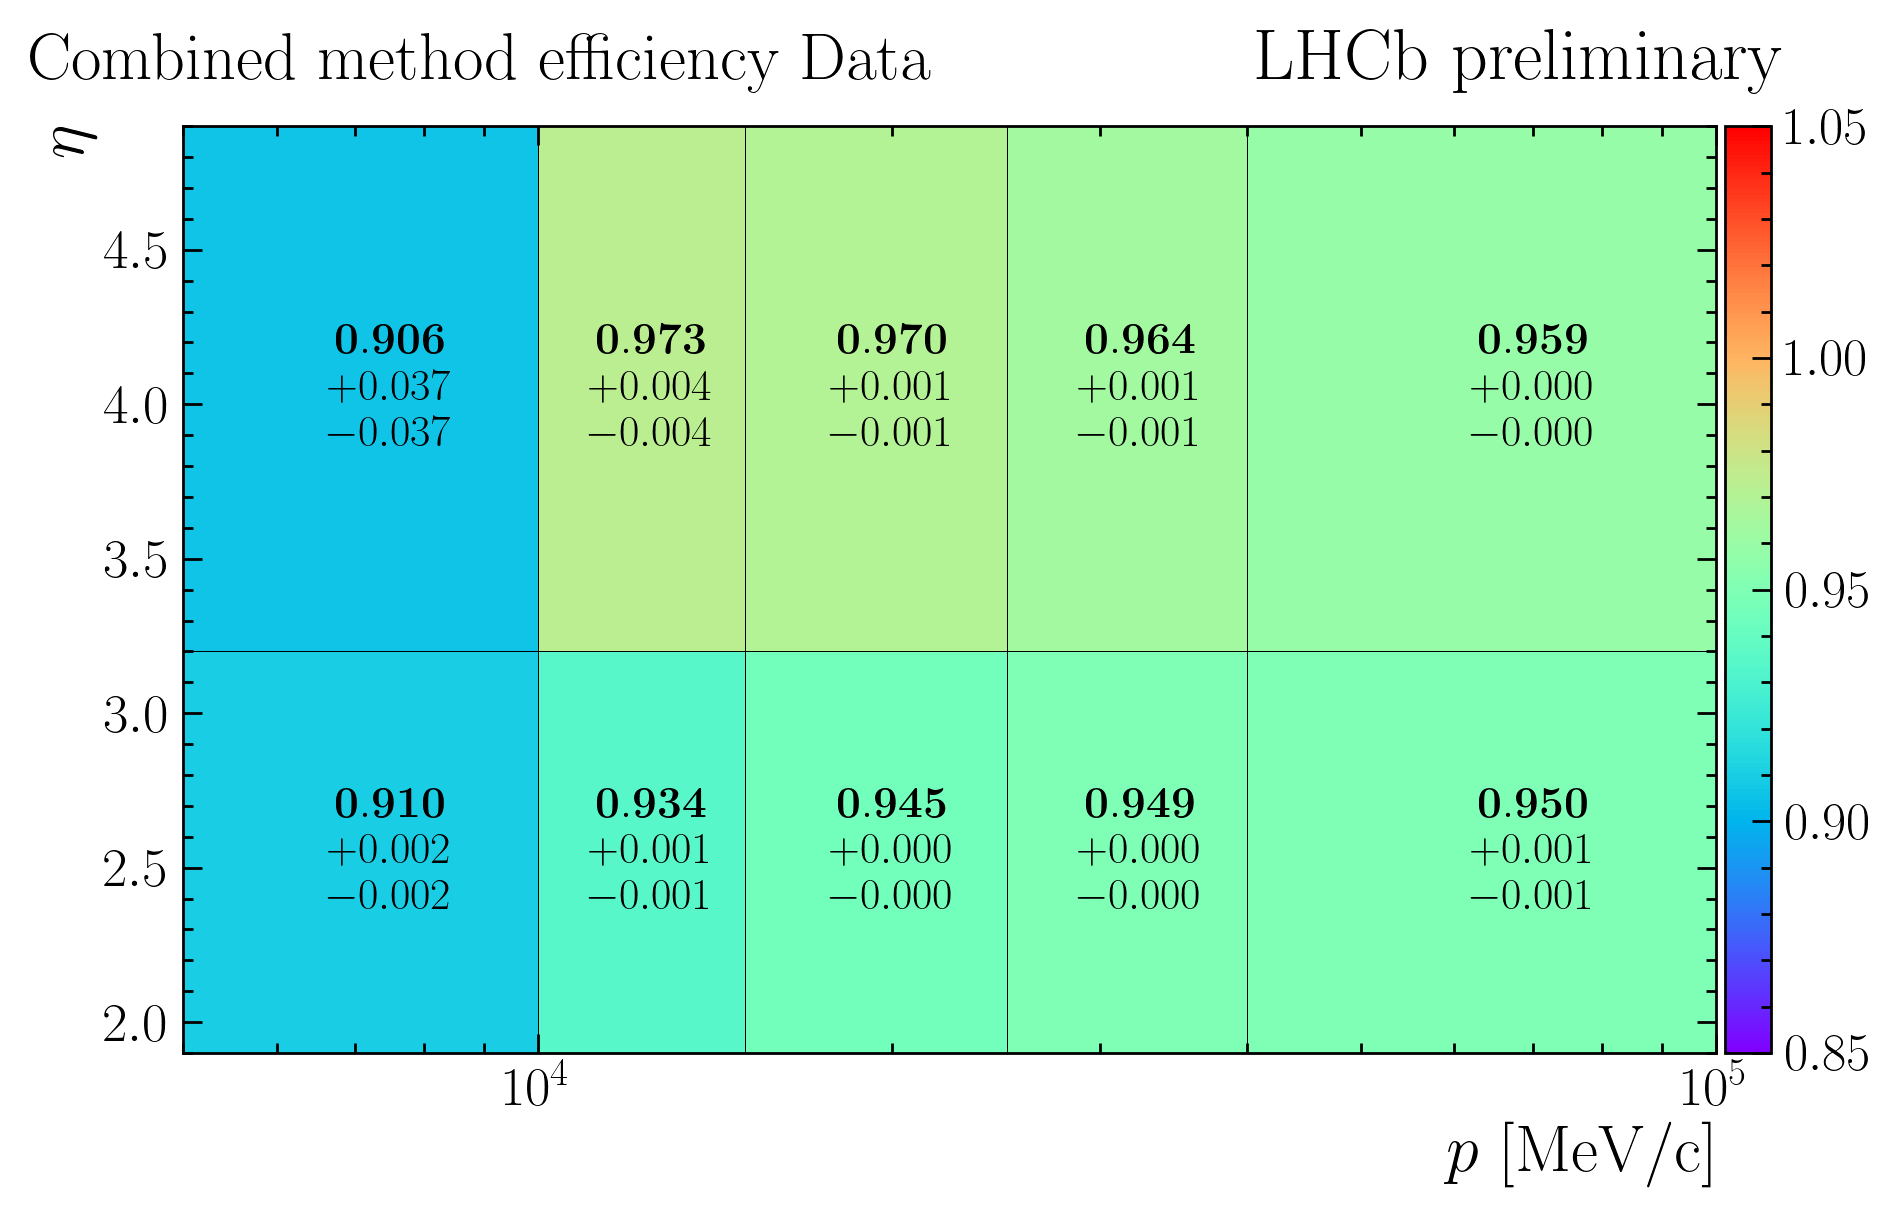
\includegraphics[width=1.0\textwidth]{Plots/trackEff_Data__2024_Block1_Combined_P-ETA.png}
    \end{subfigure}%
    \begin{subfigure}{0.5\textwidth}
      \centering
      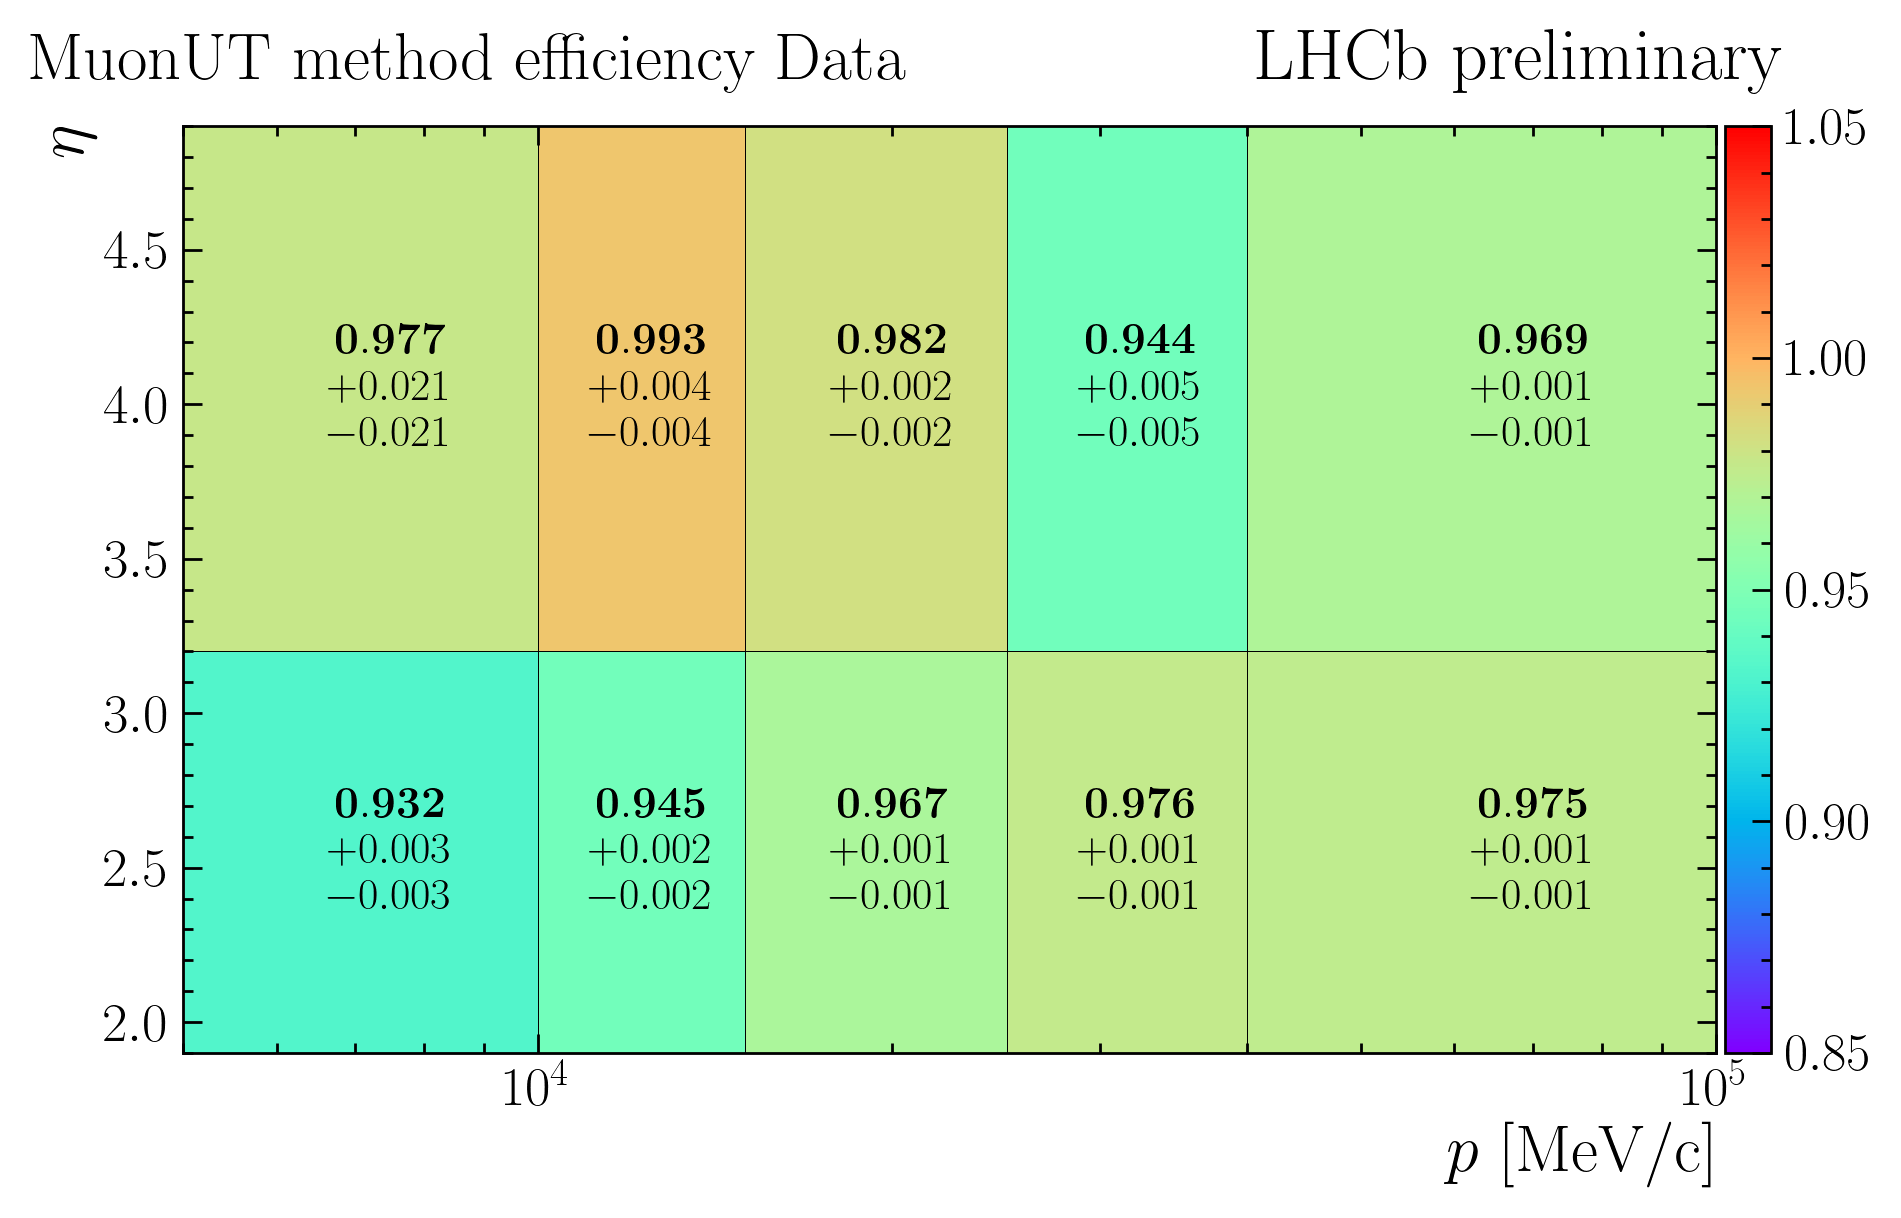
\includegraphics[width=1.0\textwidth]{Plots/trackEff_Data__2024_Block1_MuonUT_P-ETA.png}
    \end{subfigure}
  \end{figure}
  \begin{itemize}
    \item{Discrepancies are a lot larger in data than in MC, around $2\%$}
    \item{Bin $(0, 1)$ has a large discrepancy, but so are the (statistical) uncertainties}
  \end{itemize}
\end{frame}

\begin{frame}{Tracking efficiencies}
  \vspace{0.0cm}
  \begin{figure}[htb]
    \centering
    \begin{subfigure}{0.5\textwidth}
      \centering
      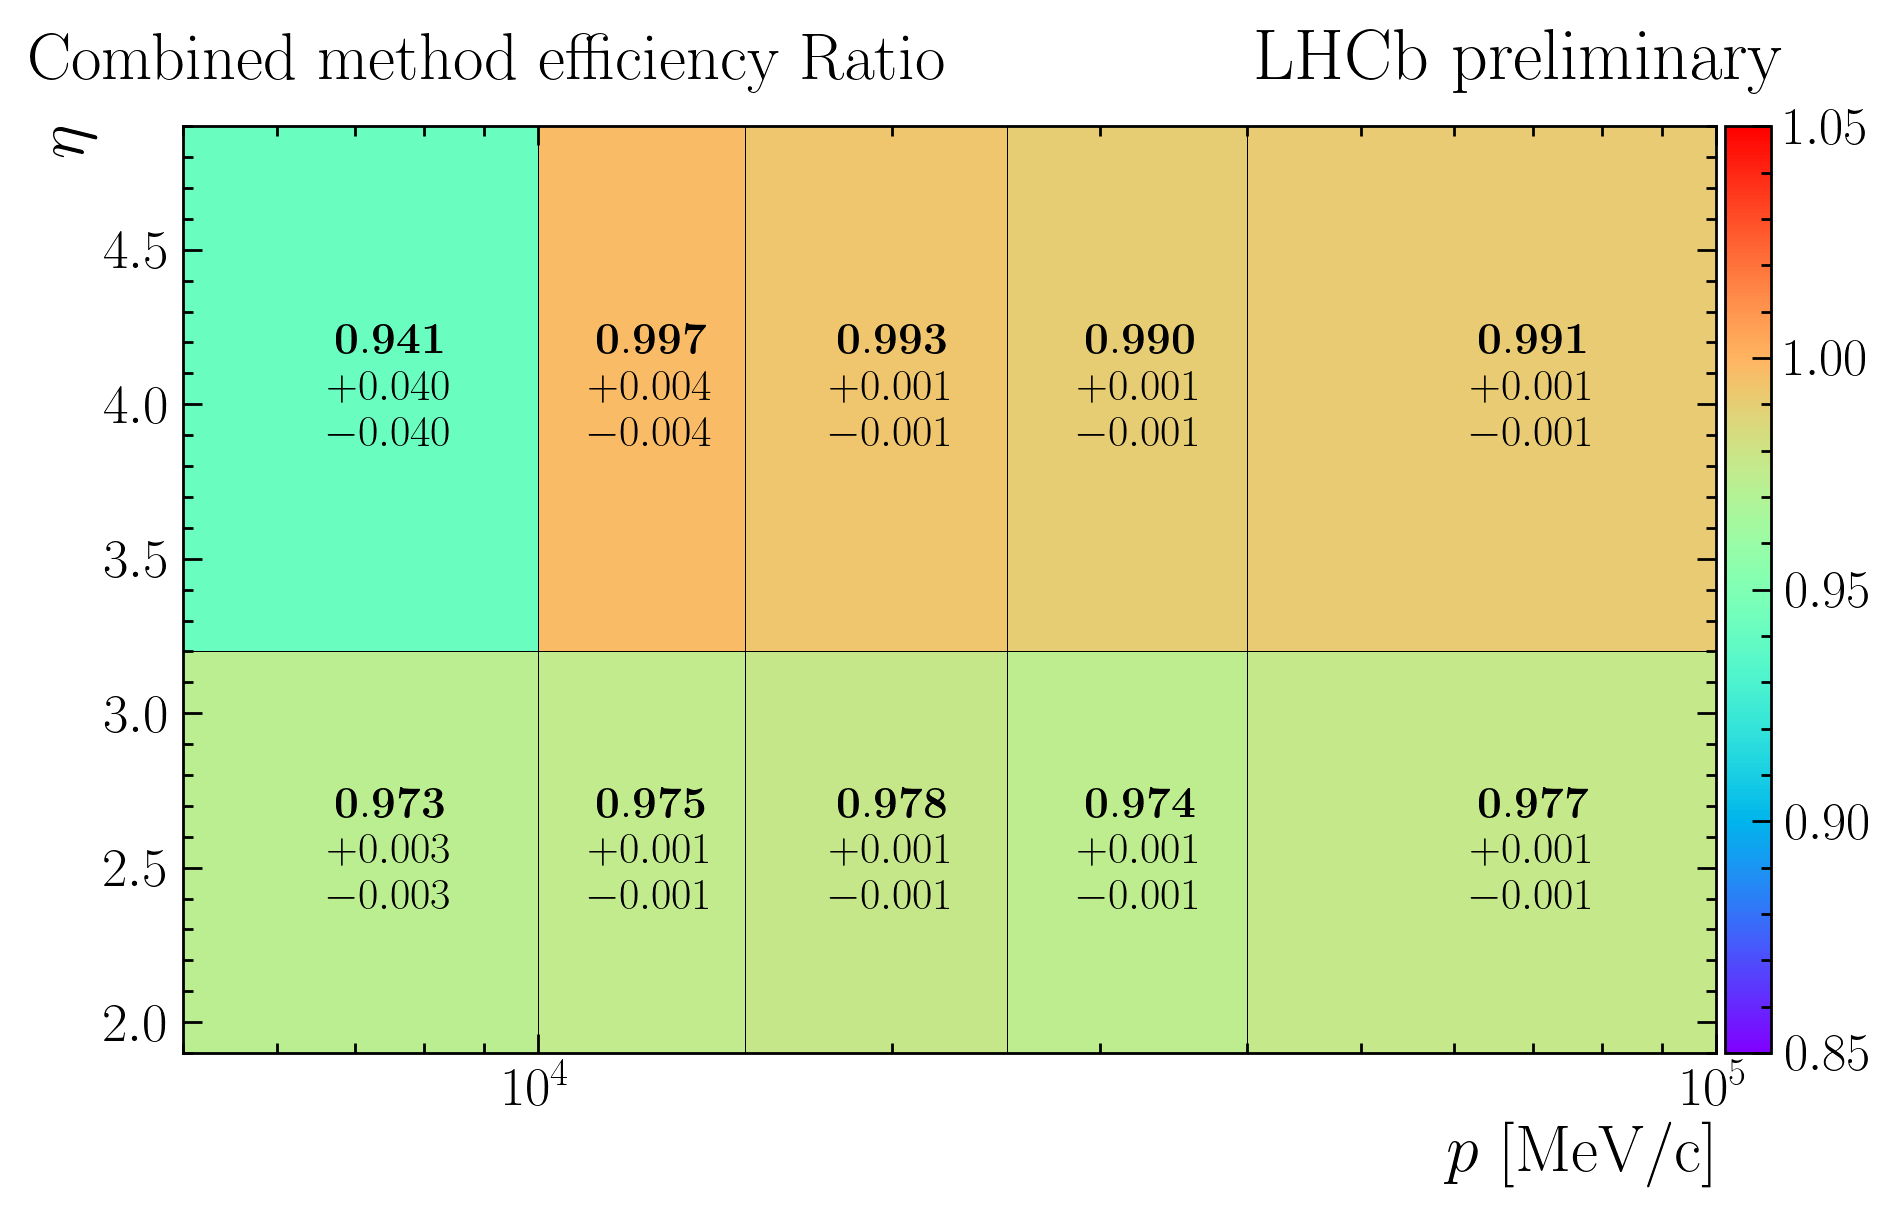
\includegraphics[width=1.0\textwidth]{Plots/trackEff_Ratio_Sim10d_2024_Block1_Combined_P-ETA.png}
    \end{subfigure}%
    \begin{subfigure}{0.5\textwidth}
      \centering
      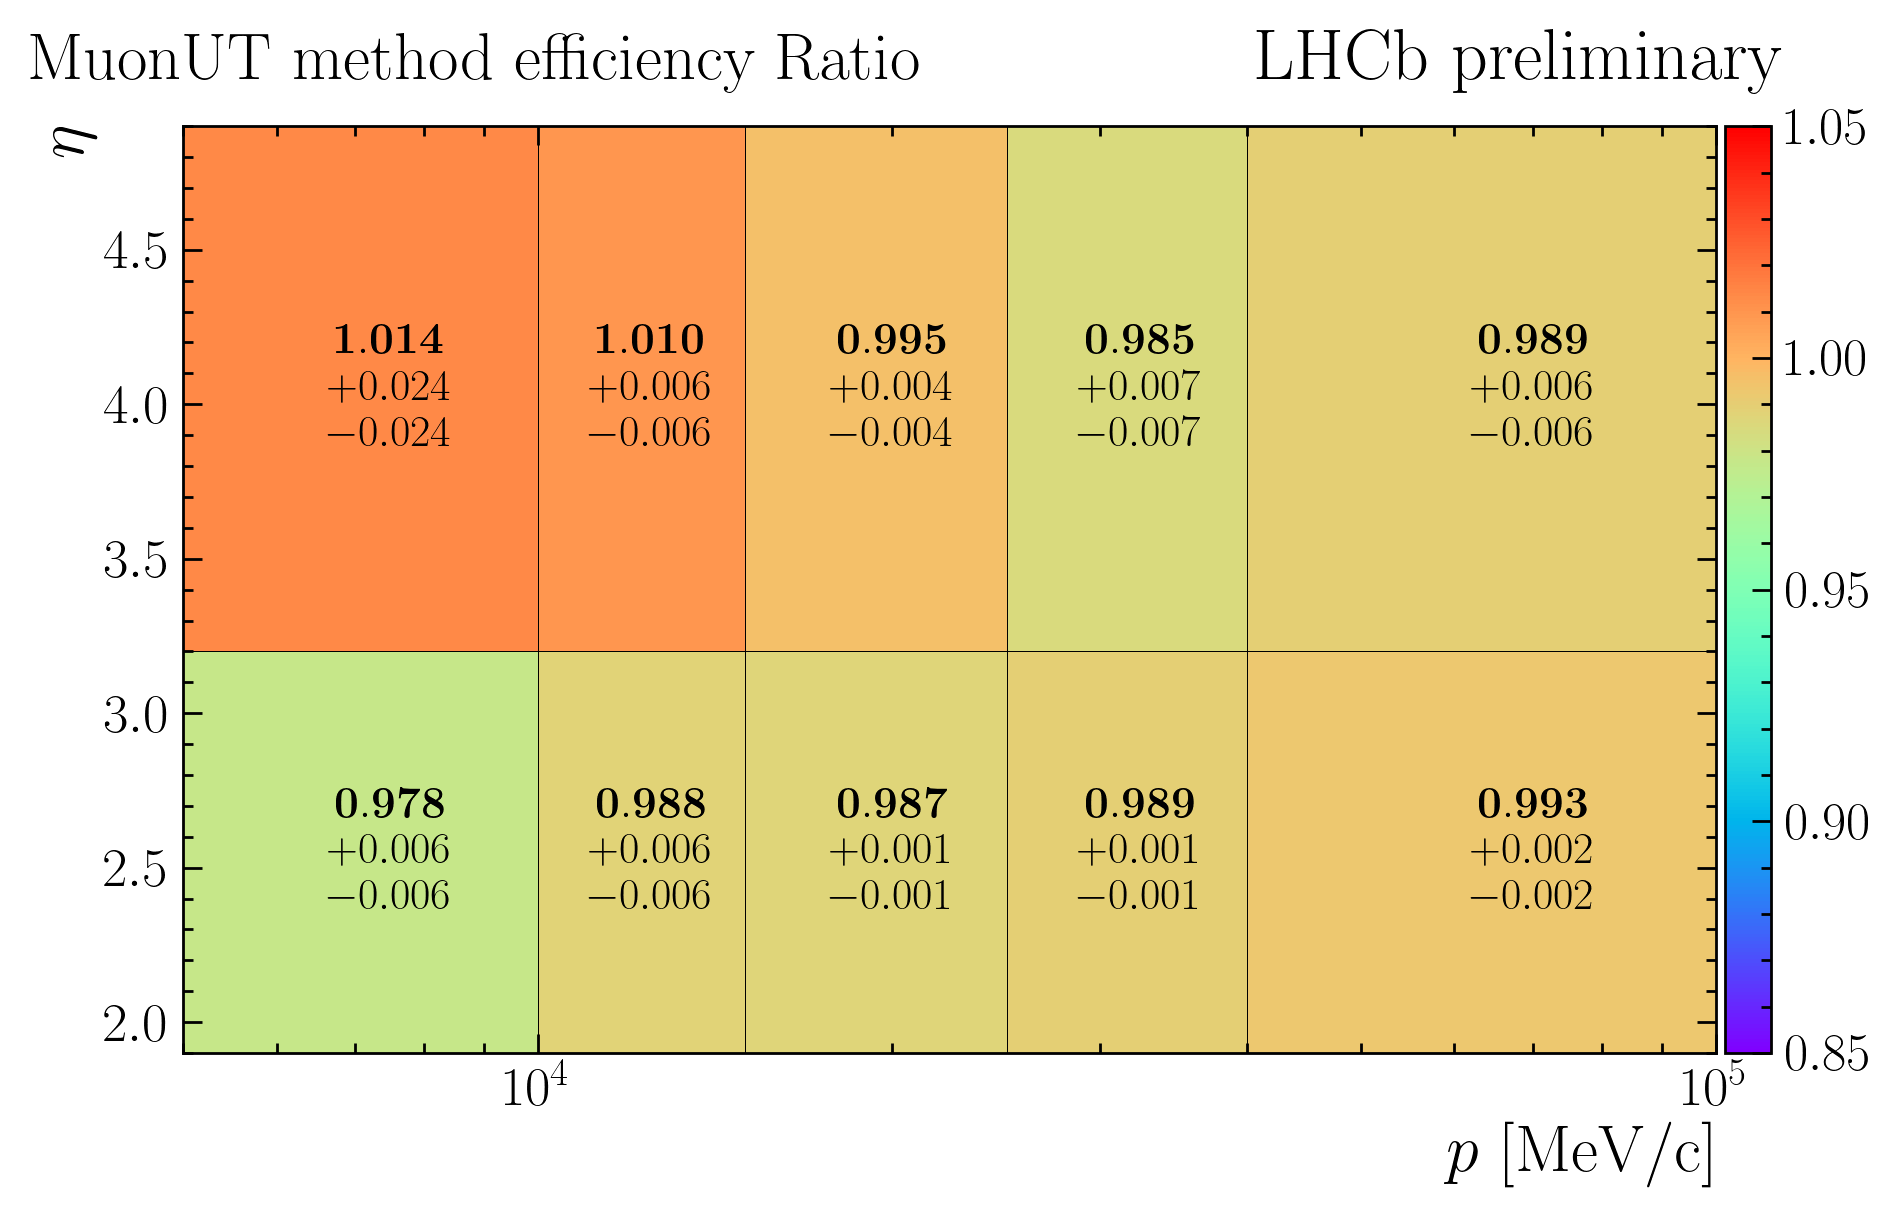
\includegraphics[width=1.0\textwidth]{Plots/trackEff_Ratio_Sim10d_2024_Block1_MuonUT_P-ETA.png}
    \end{subfigure}
  \end{figure}
  \begin{itemize}
    \item{However, when looking at the ratio, the discrepancies are mostly around $1\%$}
    \item{Bin $(0, 1)$ has a large discrepancy due to large uncertainties...}
    \item{... but apart from this bin, the largest discrepancy is $1.5\%$}
  \end{itemize}
\end{frame}

\begin{frame}{Summary and next steps}
  \vspace{0.0cm}
  \begin{itemize}
    \setlength\itemsep{0.7em}
    \item{Tweaks to TrackCalib2 to address fit biases/stability}
    \item{Fit performed on both data and MC}
    \item{Combined and MuonUT discrepancies are around $1$--$1.5\%$}
    \item{Discussion: Are these discrepancies significant?}
    \begin{enumerate}
      \item{I agree there are systematic differences between the Combined and MuonUT methods}
      \item{But the bins with largest differences also have huge statistical uncertainties...}
      \item{... so assigning a systematic of $1.0\%$ or $1.5\%$ seems reasonable to me}
    \end{enumerate}
    \item{Next steps:}
    \begin{enumerate}
      \item{Float-point precision issues in unbinned fits}
      \item{More thinking about other effects that can bias the efficiencies}
    \end{enumerate}
  \end{itemize}
  \vspace{0.3cm}
  \begin{center}
    \Huge Thanks for listening!
  \end{center}
\end{frame}

\end{document}
